% To familiarize yourself with this template, the body contains
% some examples of its use.  Look them over.  Then you can
% run LaTeX on this file.  After you have LaTeXed this file then
% you can look over the result either by printing it out with
% dvips or using xdvi.
%

\documentclass[twoside]{article}
%\usepackage{soul}
\usepackage{./lecnotes_macros}


\begin{document}
%FILL IN THE RIGHT INFO.
%\lecture{**LECTURE-NUMBER**}{**DATE**}{**LECTURERS**}{**SCRIBE**}
\lecture{5}{The Boomerang Attack}{Maria Francis and M. V. Panduranga Rao}{Gautam Singh}{24 March 2025}
%\footnotetext{These notes are partially based on those of Nigel Mansell.}

%All figures are to be placed in a separate folder named ``images''

% **** YOUR NOTES GO HERE:

This set of notes explains the original boomerang attack described in David
Wagner's 1999 paper.

\section{Introduction}
The boomerang attack is based on differential cryptanalysis. The main strength
of this attack is in the fact that preventing high probability differentials
does not make a cipher secure. According to the authors, symmetric ciphers at
the time were designed to restrict high probability differentials. Designers
would appeal to a ``folk theorem'', which states that if \(p\) is an upper bound
on the probability of any differential characteristic of the cipher, then
\(\frac{1}{p}\) texts are required to break it.

However, the boomerang attack disproves this theorem. In particular, if the best
characteristic for half of the rounds of the cipher has probability \(q\), then
the boomerang attack requires \(\cO\brak{q^{-4}}\) chosen texts. The bound would
then be surpassed if \(q^{-4} << p^{-1}\). It is worth mentioning that the
(unrelated) technique of \emph{impossible differentials} also disproves this
``folk theorem''.

\section{An Overview of the Boomerang Attack}

The boomerang attack aims to generate a quartet halfway though the cipher as
shown in \autoref{fig:boomerang-quartet}. Suppose \(E\) represents the
encryption operation. Then, we decompose the cipher into two halves \(E = E_1
\circ E_0\). Let \(\Delta \rightarrow \Delta^*\) be a differential
characteristic for \(E_0\) and \(\nabla \rightarrow \nabla^*\) be a differential
characteristic for \(E_1^{-1}\).

\begin{figure}[!ht]
    \centering
    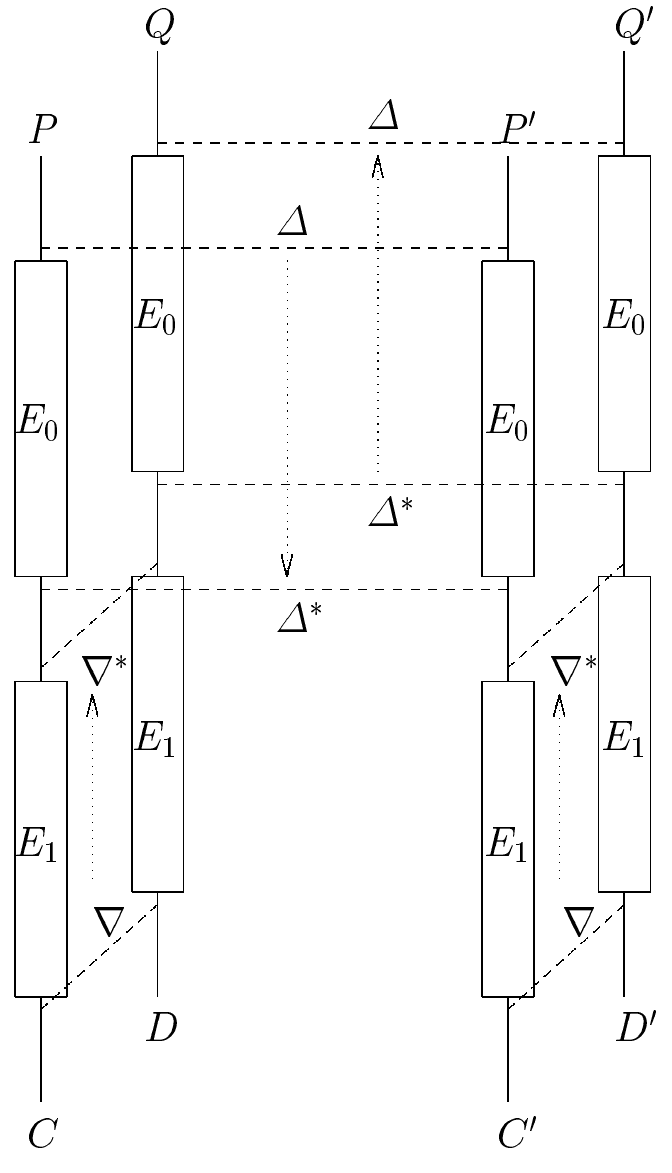
\includegraphics[width=0.2\textwidth]{images/boomerang_quartet.png}
    \caption{A schematic of the basic boomerang attack.}
    \label{fig:boomerang-quartet}
\end{figure}

The basic idea of the boomerang attack is to generate a quartet \(P, P^\prime,
Q, Q^\prime\) with ciphertexts \(C, C^\prime, D, D^\prime\) respectively such
that \(P, P^\prime\) follow the characteristic for \(E_0\) and the pairs \(P,
Q\) and \(P^\prime, Q^\prime\) follow the characteristic for \(E_1^{-1}\). Then,
the authors claim the pair \(Q, Q^\prime\) is set up to use the characteristic
\(\Delta^* \rightarrow \Delta\) for \(E_0^{-1}\). This is because

\begin{align}
    E_0\brak{Q} \oplus E_0\brak{Q^\prime} &= E_0\brak{P} \oplus E_0\brak{P^\prime} \oplus E_0\brak{P} \oplus E_0\brak{Q} \oplus E_0\brak{P^\prime} \oplus E_0\brak{Q^\prime} \\
    &= E_0\brak{P} \oplus E_0\brak{P^\prime} \oplus E_1^{-1}\brak{C} \oplus E_1^{-1}\brak{D} \oplus E_1^{-1}\brak{C^\prime} \oplus E_1^{-1}\brak{D^\prime} \\
    &= \Delta^* \oplus \nabla^* \oplus \nabla^* = \Delta^*.
    \label{eq:qq-e0}
\end{align}

From \eqref{eq:qq-e0}, we see that \(Q, Q^\prime\) will also follow the same
characteristic as \(P, P^\prime\), which shows the ``boomerang''. A \emph{right
quartet} is one where all the four characteristics mentioned above hold for
their respective pairs. To generate this quartet, one can choose an arbitrary
\(P\) and set \(P^\prime = P \oplus \Delta\). After obtaining \(C, C^\prime\)
with two chosen-plaintext queries, we can generate \(D = C \oplus \nabla\) and
\(D^\prime = C^\prime \oplus \nabla\). Finally, we obtain \(Q, Q^\prime\) with
two adaptive chosen-ciphertext queries. After generating sufficiently many right
quartets, a suitable counting scheme may be used for cryptanalysis or an attack
distinguishing the cipher from a truly random function may be carried out.

We will now describe the working of COCONUT98 and the boomerang attack on it.

\section{Cryptanalysis of COCONUT98}
The COCONUT98 cipher uses decorrelation techniques to admit no high probability
differentials over the entire cipher. However, the boomerang attack still works
and is able to break this cipher.

\subsection{The COCONUT98 Algorithm}
COCONUT98 uses a 256-bit key \(K = \brak{K_1, \ldots, K_8}\). The key schedule
is shown in \autoref{fig:coconut-key-schedule}.

\begin{table}[!ht]
    \centering
    \begin{tabular}{|c|c|c|c|c|c|c|c|c|c|}
        \hline
        \(i\) & 1 & 2 & 3 & 4 & 5 & 6 & 7 & 8 \\
        \hline
        \(k_i\) & \(K_1\) & \(K_1 \oplus K_3\) & \(K_1 \oplus K_3 \oplus K_4\) &
        \(K_1 \oplus K_4\) & \(K_2\) & \(K_2 \oplus K_3\) & \(K_2 \oplus K_3
        \oplus K_4\) & \(K_2 \oplus K_4\) \\
        \hline
    \end{tabular}
    \caption{Key schedule of COCONUT98.}
    \label{fig:coconut-key-schedule}
\end{table}

The last four words of the key are used in the decorrelation module

\begin{equation}
    M\brak{xy} = \brak{xy \oplus K_5K_6} \times K_7K_8 \bmod{\textrm{GF}\brak{2^{64}}}
    \label{eq:coconut-m}
\end{equation}

where \(xy\) denotes the concatenation of the 32-bit words \(x\) and \(y\) and
\(\textrm{GF}\brak{2^{64}}\) denotes the Galois Field of size \(2^{64}\).

Now, we can build the Feistel network. Suppose that \(c\) is a public 32 bit
constant, \(ROL_{11}\brak{\cdot}\) represents left rotation by 11 bits and \(S :
\bZ_2^8 \rightarrow \bZ_2^{24}\) is a fixed S box. Then, the \(i\)-th round
function \(F_i\) is given by

\begin{align}
    \phi\brak{x} &= x + 256\cdot S\brak{x \bmod 256} \bmod 2^{32} \\
    F_i\brak{\brak{x, y}} &= \brak{y, x \oplus \phi\brak{ROL_{11}\brak{\phi\brak{y \oplus k_i}} + c \bmod 2^{32}}} \\
    \Psi_i &= F_{4i+4} \circ F_{4i+3} \circ F_{4i+2} \circ F_{4i+1}
\end{align}

and COCONUT98 is defined as \(\Psi_1 \circ M \circ \Psi_0\). Thus, there are
four Feistel rounds before and after the decorrelation module.

\subsection{Differential Characteristics of COCONUT98}
Every differential \(\delta \rightarrow \delta^*\) over \(M\) has an average
probability of \(\frac{1}{2^{64} - 1}\), where \(\delta, \delta^* \neq 0\). This
is the reason why COCONUT98 does not admit high probability differentials. This
makes it a perfect candidate to demonstrate the strength of the boomerang
attack.

Suppose \(e_j = 2^j\) for \(0 \le j < 32\) (we consider 0-based subscripts here
to better model the left rotation). An important differential characteristic for
one round of COCONUT98 is that \(e_j \rightarrow e_{j + 11}\) with probability
approximately \(\frac{1}{2}\) when \(j \in J =
\cbrak{8,9,\ldots,19,20,29,30,31}\). To see how, we can write \(x \xmapsto{\phi}
\brak{x + a \bmod 2^{32}}\) and the overall effect of \(F\) is \(x \xmapsto{F}
\brak{x + a \bmod 2^{32}} + b \bmod 2^{32}\) which can be written as \(x + c
\bmod 2^{32}\), where \(c = a + b\). In other words, there is effectively only
one carry happening for bits in \(J\). Empirically, the probabilities are
smaller than \(\frac{1}{2}\) for some values of \(j\). For instance, the
probabilities are \(0.47,0.44,0.38\) for \(j = 18,19,20\) and \(0.47,0.44\) for
\(j = 29,30\).

This observation enables us to write four-round characteristics for COCONUT98
such as 

\begin{equation}
    \brak{e_{19}, e_{18} \oplus e_8} \rightarrow \brak{e_{18} \oplus e_{8}, e_{29}} \rightarrow \brak{e_{29}, e_{18}} \rightarrow \brak{e_{18}, 0} \rightarrow \brak{0, e_{18}}
    \label{eq:coconut-char}
\end{equation} 

with probability \(0.83 \cdot 2^{-4} \approx 2^{-4.3}\).

We now have our differentials for the two halves of the cipher, but we have to
account for the decorrelation module. The authors use the crucial idea that
\(M\) is affine to make the boomerang attack work. For any fixed key, the
decorrelation module \(M\) becomes affine (of the form \(y = mx + c\)) and thus
has characteristics \(\nabla^* \rightarrow M^{-1}\brak{\nabla^*}\) with
probability 1. Thus, by absorbing \(M\) in either \(E_0\) or \(E_1\), there will
be no change in the probabilities of the respective characteristics over half
the rounds. In other words, the attacker need not know the exact value of
\(M^{-1}\brak{\nabla^*}\), since it depends only on the key.

An estimate of the success probability for this attack is 

\begin{equation}
    p \approx \sum_{\Delta^*}\Pr\sbrak{\Delta \rightarrow \Delta^* \textrm{ by } \Psi_0}^2 \cdot \sum_{\nabla^*}\Pr\sbrak{\nabla \rightarrow \nabla^* \textrm{ by } \Psi_1^{-1}}^2.
    \label{eq:coconut-p-approx}
\end{equation}

We do not need to know that value of \(\nabla^*\) in advance because we only
require that the difference after decrypting by \(\Psi_1\) is same in the pairs
\(P, Q\) and \(P^\prime, Q^\prime\). A similar argument holds for \(\Delta^*\).
The authors find empiricially that \(\Delta = \nabla = \brak{e_{10}, e_{31}}\)
gives \(p \approx 0.023 \cdot 0.023 \approx \frac{1}{1900}\).

\subsection{The Boomerang Attack on COCONUT98}
The authors use a 1-R attack on COCONUT98, where the success criterion is \(Q
\oplus Q^\prime = \brak{?, e_{31}}\) with \(?\) representing an arbitrary word.
This doubles the success probability to \(\frac{1}{950}\). Clearly, we can use
\(950 \cdot 4 = 3800\) adaptive chosen plaintext/ciphertext (ACPC) queries to
distinguish COCONUT98 from an ideal cipher.

For a key recovery attack, notice that we can generate 16 right quartets in
about \(16 \cdot 950 \cdot 4\) ACPC. With a very high signal to noise ratio, the
quartets should be filtered out effectively. To peel of the first (and last)
rounds, we exhaustively search \(K_1\). Notice that 16 quartets are enough since
the XOR difference after one round will be \(\brak{e_{31}, 0}\), which holds for
half of the wrong key values since the probability of this characteristic is
\(\frac{1}{2}\). Using the 32 pairs from each of the 16 quartets should be
enough to uniquely identify \(K_1\) and similarly \(K_2 \oplus K_4\). Now we can
repeat this attack on the peeled-off cipher similarly with more ACPC to generate
some more quartets. Notice that with each peel, the characteristic probability
will increase and fewer ACPC are needed to get enough quartets.

The complexity of this attack is about \(16 \cdot 950 \cdot 4 + 8 \cdot 144
\cdot 4 + \ldots \approx 2^{16}\) ACPC. Additionally, this attack requires \(8
\cdot 2 \cdot 32 \cdot 2^{32} = 2^{41}\) offline computations of the \(F\)
function. Converting this to a known-plaintext attack will increase the
complexity to \(2^{52}\) texts. Since offline computations are one-time, this
attack is practical.

The authors propose a few ways to strengthen COCONUT98. One way is to use more
rounds to weaken the characteristic probabilities over half the cipher (for
instance, using 16 rounds instead of 4). Another approach could be to use the
decorrelation module after each Feistel round.

\end{document}
